%%%%%%%%%%%%%%%%%%%%%%%%%%%%%%%%%%%%%%
% 
% TODO:
% 1. Figure out a smoother way for the document to flow onto the next page.
% 3. Add more icon options 
% 4. Fix hacky left alignment on contact line
% 5. Remove Hacky fix for awkward extra vertical space
% 
%%%%%%%%%%%%%%%%%%%%%%%%%%%%%%%%%%%%%%
%
% CHANGELOG:
%
%%%%%%%%%%%%%%%%%%%%%%%%%%%%%%%%%%%%%%%
%
% Known Issues:
% 1. Overflows onto second page if any column's contents are more than the vertical limit.
%%%%%%%%%%%%%%%%%%%%%%%%%%%%%%%%%%%%%%
%%Icons:
%%Main: https://icons8.com/icons/carbon-copy
%%%%%%%%%%%%%%%%%%%%%%%%%%%%%%%%%%

\documentclass[]{plushcv}
\usepackage{fancyhdr}
\pagestyle{fancy}
\fancyhf{}
\begin{document}

%%%%%%%%%%%%%%%%%%%%%%%%%%%%%%%%%%%%%%
%
%     MY CV
%
%%%%%%%%%%%%%%%%%%%%%%%%%%%%%%%%%%%%%%

\namesection{Andres}{Acuña Marrroquín}{}

{\contactline{
\href{mailto:andres.acunamarroquin@gmail.com}{andres.acunamarroquin@gmail.com}}{\href{https://www.github.com/Andres-AM}{Andres-AM}}
{\href{tel:+41782281628}{078 228 16 28}}}
\hfill 
\smash{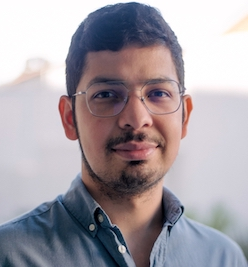
\includegraphics[width=3cm]{Andres.jpeg}}
\sectionsep
\sectionsep
\sectionsep


% {\contactline
% {\href{mailto:andres.munoztord@mailbox.org}{andres.acunamarroquin@gmail.com}}
% {\href{https://www.github.com/Andres-AM}{Andres-AM}}
% {\href{https://www.linkedin.com/in/andr%C3%A9s-acu%C3%B1a-marroqu%C3%ADn/}{Andres AM}}
% {\href{tel:+41782281628}{078 228 16 28}}}
% \hfill 
% \smash{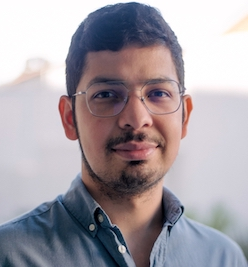
\includegraphics[width=3cm]{Andres.png}}
% \sectionsep
% \sectionsep
% \sectionsep
%%%%%%%%%%%%%%%%%%%%%%%%%%%%%%%%%%%%%%
%
%     COLUMN ONE
%
%%%%%%%%%%%%%%%%%%%%%%%%%%%%%%%%%%%%%%

\begin{minipage}[t]{0.70\textwidth} 


%%%%%%%%%%%%%%%%%%%%%%%%%%%%%%%%%%%%%%
%     EXPERIENCE
%%%%%%%%%%%%%%%%%%%%%%%%%%%%%%%%%%%%%%
\sectionsep

\section{Experience}



\runsubsection{VERACYTE INC.}
\descript{| Principal Biostatistician }
\location{Part-time: May 2019 – August 2022 | Marseille, France}
\begin{tightemize}
\sectionsep
\sectionsep
\item Performed data analysis to identify trends in customer behavior.
\item Conducted research to develop new methods for data analysis.
\item Developed data models to predict customer behavior that produced a 10\% increase in revenue.
\item Created visualizations to communicate findings to stakeholders.
\item Implemented data-driven solutions to improve customer engagement.
\item Collaborated with cross-functional teams to create and deploy machine learning algorithms, resulting in a 25\% reduction in customer churn.


% \item Managed Linux servers for Data Science team.
% \item Developed ETL for on-premise PostgreSQL Data Warehouse.
% \item Built ML pipelines to implement predictive models to detect fraud in clients behavior.
% \item Demonstrated knowledge and execution of application programming interface development and test automation.
% \item Updated data streaming processes for a reduction in redundancy and pipeline automation using CI/CD principles.
% \item Utilized analytical and technical expertise to provide insights and proposals to support business improvements.
\end{tightemize}
\sectionsep

\runsubsection{CICAD Organisation}
\descript{| Data Engineer }
\location{Part-time: October 2022 – Present | Geneva, Switzerland}
\begin{tightemize}
\sectionsep
\item Worked closely with analysts across departments to design, build and deploy various initiatives within the data platform.
\item Developed, deployed and maintained data services using R and PostgreSQL.
\item Prepared and presented analysis for trimestrial reports.
\item Designed best practices to support continuous process automation for data ingestion and data pipeline workflows.
\item Automated amalgamation of data from spreadsheet revenue calculations and PDF reports reducing month end processing time from 2 days to 4 minutes.
\end{tightemize}
\sectionsep




\runsubsection{FlowBank}
\descript{| R Developer/ Data Engineer}
\location{April 2022 – January 2023 | Geneva, Switzerland}
\begin{tightemize}
\sectionsep
\item Developed and implemented complex statistical models in R, resulting in a 15\% increase in accuracy for predicting customer behavior.
\item Designed and maintained a data visualization dashboard in R, which allowed for easy monitoring of key performance indicators and resulted in a 20\% reduction in reporting time.
\item Conducted thorough data analysis, resulting in the identification of cost-saving opportunities that resulted in a 5\% reduction in expenses.
\item Managed Linux servers for the Data Science team and designed best practices to support continuous process automation for data ingestion and data pipeline workflows.

\end{tightemize}
\sectionsep

\runsubsection{University of Geneva}
\descript{| Lecturer in Statistics }
\location{Part-time: September 2020 – January 2023 | Geneva, Switzerland}
\begin{tightemize}
\sectionsep
\item Taught theoretical aspect of statistical modelling.
\item Created freely available data wrangling
\href{https://Andres-AM.github.io/Hitchhikers_guide_to_the_brain/}{\underline{tutorials and workshops}} in R and Python.
\end{tightemize}
\sectionsep

\sectionsep
\runsubsection{Campus Biotech}
\descript{| Graduate Research Assistant in Neuroscience}
\location{August 2019 – November 2021 | Geneva, Switzerland}
% \vspace{\topsep} % Hacky fix for awkward extra vertical space
\begin{tightemize}
% \sectionsep
\item Developed and implemented computational models of neural systems.
\item Conducted research on the mechanisms of neural computations.
\item Investigated the dynamics of neural circuits.
\item Analyzed the data from neural recordings.
\item Applied new methods of model falsification and parameter recovery in a theory-driven approach to computational modelling. \href{https://github.com/Andres-AM/Computational-Modelling}{\underline{CompModeling}}.
\end{tightemize}
\sectionsep

% \item Used various statistical methods to analyze large
% scale dataset: Hierarchical Bayesian modeling,
% Multivariate pattern analysis, and model-free reinforcement
% learning.
% \item Researched and studied human health conditions
% and behavior.
% \item Processed terabytes of raw MRI data for a large scale of
% longitudinal clinical trials.
% \item Managed neuromedical data according to
% the BIDS regulatory compliance specifications.
% \item Set up and maintained a Linux cluster for
% scientific computing for the lab.
% \item Helped other lab members with their analysis and
% created online tools for data visualization.



% \sectionsep
% \runsubsection{GENEVA UNIVERSITY NEUROCENTER}
% \descript{| Internship in Computational Neuroscience }
% \location{August July 2019 – December 2019 | Geneva, Switzerland}
% \begin{tightemize}
% % \sectionsep
% \item Processing and analysis of EEG/ERP signal.
% \item Training in the notions of model falsification and
% parameter recovery in a theory-driven approach to computational modelling. 

% \sectionsep


% \sectionsep
% \runsubsection{UNIVERSITY OF GENEVA}
% \descript{| UNDERGRADUATE RESEARCH ASSISTANT IN PSYCHOLOGY}
% \location{February September 2016 – August 2017 | Geneva, Switzerland}
% \begin{tightemize}
% % \sectionsep
% \item Collecting data for a cognitive neuroscience experiment.

% \end{tightemize}
% \sectionsep










% \section{Languages}
% \runsubsection{}
% \location{Fluent \phantom{eeeeeeeeeeeeeeeeeeeeeeeeeeeeeeeeeeeeeeeee} Basic}
% \descript{English | French | Spanish \phantom{eeeeeeeeeeeeeeeee} German | Italian | Portuguese}



%%%%%%%%%%%%%%%%%%%%%%%%%%%%%%%%%%%%%%
%     AWARDS
%%%%%%%%%%%%%%%%%%%%%%%%%%%%%%%%%%%%%%

% \section{Awards} 
% \begin{tabular}{rll}
% 2020	     & Finalist & Lorem Ipsum\\
% 2018	     & $2^{nd}$ & Dolor Sit Amet\\
% 2015	     & Finalist  & Cras posuere\\
% \\
% \end{tabular}
% \sectionsep
%%%%%%%%%%%%%%%%%%%%%%%%%%%%%%%%%%%%%%
%
%     COLUMN TWO
%
%%%%%%%%%%%%%%%%%%%%%%%%%%%%%%%%%%%%%%

\end{minipage} 
\hfill
\begin{minipage}[t]{0.25\textwidth} 

%%%%%%%%%%%%%%%%%%%%%%%%%%%%%%%%%%%%%%
%     SKILLS
%%%%%%%%%%%%%%%%%%%%%%%%%%%%%%%%%%%%%%
\sectionsep
\sectionsep
\sectionsep
\sectionsep

\subsection{Skills}
\sectionsep
\runsubsection{}
\descript{Programming}
\location{Proficient:}
\justified{ \textbf{
R \textbullet{} Python \textbullet{} BASH \textbullet{} SQL}}
\sectionsep

\location{Experienced:}
\justified{ \textbf{MATLAB \textbullet{}  STAN  \textbullet{} JavaScript  }}\\
\sectionsep

\runsubsection{}
\descript{Libraries/Frameworks}
\justified{ \textbf{TensorFlow \textbullet{}
Scikit-Learn \textbullet{}
Pandas \textbullet{}
Spark MLib \textbullet{}
PyTorch \textbullet{}
Matplotlib\textbullet{} 
Numpy \textbullet{} Dash \textbullet{} 
Tidyverse \textbullet{} BRMS \textbullet{} Rstan \textbullet{} Caret \textbullet{}
Glmnet \textbullet{}  \textbullet{} Node.js }}
\sectionsep

\runsubsection{}
\descript{Tools/Paradims}
\justified{ \textbf{Git \textbullet{} AWS: S3, Sagemaker, Glue \textbullet{} MlOps \textbullet{} Azure DevOps}}

\sectionsep

%%%%%%%%%%%%%%%%%%%%%%%%%%%%%%%%%%%%%%
%     EDUCATION
%%%%%%%%%%%%%%%%%%%%%%%%%%%%%%%%%%%%%%
\sectionsep
\subsection{Education} 
\sectionsep
\descript{Master of Neurosciences | Geneva Neurocenter}
\location{\textbf{Sept 2018 - March 2020 | Switzerland}}
\justified{\locationthir{Coursework in Reinforcement learning, AI, Data science and Neuroimaging. GPA: 3.85}}
% \locationsec{ Cum. GPA: 3.85 / 4.0 }

\sectionsep
\descript{Complementary Studies in Data Science | UMass Amherst}
\location{Sept 2017 - June 2018 | MA, USA}
\justified{\locationthir{
Received Global Fellow full scholarship.
Capstone project: Detecting planets via transits. SQL database querying.}}
\sectionsep

\sectionsep
\descript{Bachelor of Science | University of Geneva}
\location{Sept 2014 - June 2017 | Switzerland}
\justified{\locationthir{Relevant coursework completed in statistics and scientific programming.}}
\sectionsep

%%%%%%%%%%%%%%%%%%%%%%%%%%%%%%%%%%%%%%
%     COURSEWORK
%%%%%%%%%%%%%%%%%%%%%%%%%%%%%%%%%%%%%%
\sectionsep
\runsubsection{}
\descript{Coursework}
\justified{ \textbf{Algorithms \textbullet{}
Data Mining \textbullet{} Machine Learning \textbullet{} Artificial Intelligence \textbullet{}
Linux System Administration \textbullet{} 
Visualization For Scientific Data \textbullet{}
Database Management Systems \textbullet{}
Object Oriented Programming \textbullet{}
Scripting Languages and Web Tech}}
\sectionsep
\sectionsep

% \runsubsection{}
% \descript{Publications}
% \href{https://github.com/Andres-AM/publications}{\underline{My recent publications}}



\end{minipage} 
\clearpage
\begin{minipage}[t]{0.70\textwidth} 
\sectionsep
\sectionsep
\sectionsep
\sectionsep
\sectionsep
\sectionsep
\sectionsep
\sectionsep




%%%%%%%%%%%%%%%%%%%%%%%%%%%%%%%%%%%%%%
%     Projects
%%%%%%%%%%%%%%%%%%%%%%%%%%%%%%%%%%%%%%

\section{Projects}
\sectionsep


\runsubsection{Echarts4r}
\sectionsep
\sectionsep
\descript{| R, JavaScript - 2023 - Present}
% \location{2021}
\begin{tightemize}
\item Is an open-source R package that provides a powerful rendering engine allowing progressive rendering up to 10 million data points in realtime.
\end{tightemize}
\sectionsep


\runsubsection{Geneva R-Lunches}
\sectionsep
\descript{| R - 2023 - Present}
% \location{2021}
\begin{tightemize}
\item Multidisciplinary meetings on R at UniMail (\href{https://use-r-carlvogt.github.io/prochains-lunchs/}{\underline{presentations}}). 
\end{tightemize}
\sectionsep



\runsubsection{We Data}
\sectionsep
\descript{| R, Rust and Python - 2022 - Present}
% \location{2021}
\begin{tightemize}
\item We Data is an organization that shares knowledge on code in social sciences (\href{https://wedata.ch/}{\underline{Blog}}, \href{https://www.youtube.com/channel/UCGktdbvbc_H-JEkYYTvwRVw}{\underline{YouTube channel}}), give \href{https://github.com/we-data-ch/workshops}{\underline{workshops about statistics}}, and do coding demonstrations. 
\end{tightemize}
\sectionsep

\runsubsection{D\MakeLowercase{b}V\MakeLowercase{iewe}R}
\descript{| R, JavaScript and SQL - 2022 - present}
% \location{2021}
\begin{tightemize}
\item A shiny app that simulates a database management system featuring functions like login authentication, save/create/delete tables, add/rename columns, using either a PostgreSQL or SQLite back-end [\href{https://github.com/Andres-AM/DBMS}{\underline{DbVieweR}}].
\end{tightemize}
\sectionsep
\runsubsection{\MakeLowercase{h}B\MakeLowercase{ayes}DM}
\descript{| STAN, R and Python - 2021}
\begin{tightemize}
\item Collaborated on the Hierarchical Bayesian modeling of Decision-Making tasks library [\href{https://github.com/CCS-Lab/hBayesDM}{\underline{hBayesDM}}]. Built Q-learning algorithm for probabilistic selection task.
\end{tightemize}
\sectionsep



\runsubsection{3\MakeLowercase{d}LME\MakeLowercase{r}}
\descript{| BASH and R - 2020}
% \location{2018}
\begin{tightemize}
\item Collaborated on the AFNI's functions for 3Dimensional Linear Mixed-Effects Regression [\href{https://github.com/afni/afni/blob/ebd2aef51c27cf7684f38f580e1db832b1ccf621/src/R_scripts/3dLMEr.R}{\underline{3dLMEr}}]. Fixed residuals output image by adding bottom tolerance.
\end{tightemize}
\sectionsep

% \runsubsection{REBUND}
% \descript{| JavaScript - 2020}
% \begin{tightemize}
% \item Developed an online interactive experiment to investigate chemo sensory preferences with the Revealed Preference paradigm [\href{https://github.com/Andres-AM/Rebund}{\underline{Rebund}}].
% \end{tightemize}
% \sectionsep


% %%%%%%%%%%%%%%%%%%%%%%%%%%%%%%%%%%%%%%
% %     Publications
% %%%%%%%%%%%%%%%%%%%%%%%%%%%%%%%%%%%%%%



\section{Publications} 


\location{Does GLP-1 receptor agonist liraglutide alter food-related sensory pleasure in patients with obesity? A randomized controlled trial. \href{https://doi.org/10.21203/rs.3.rs-1722974/v1}{\underline{Paper}}}
\locationthir{Coppin, G., ACUÑA MARROQUÍN, D., Pool, Cereghetti, D., Golay, A., Sander, D., \& Pataky,  Z. Europe PMC (2022)}
\sectionsep

\location{Differential contributions of ventral striatum subregions to the motivational and hedonic components of the affective processing of the reward. \href{https://doi.org/10.1523/JNEUROSCI.1124-21.2022}{\underline{Paper}}}
\locationthir{Pool, E. R., ACUÑA MARROQUÍN, D. , Delplanque, S., Stussi, Y., Cereghetti, D., Vuilleumier, P., \& Sander, D. Journal of Neuroscience (2022)}
\sectionsep

\location{3D-printed pacifier-shaped mouthpiece for fMRI-compatible gustometers. \href{https://dx.doi.org/10.1523\%2FENEURO.0208-21.2021}{\underline{Paper}}}
\locationthir{ACUÑA MARROQUÍN, D., Coppin, G., Pool, E. R., Mermoud, C., Pataky, Z., Sander, D., \& Delplanque, S. Eneuro (2021)}
\sectionsep

\location{Early spatial attention deployment toward and away from aggressive voices. \href{https://doi.org/10.1093/scan/nsy100}{\underline{Paper}}}
\locationthir{Burra, N., Kerzel, D., ACUÑA MARROQUÍN, D., Grandjean, D., \& Ceravolo, L. Social Cognitive and Affective Neuroscience (2019)}
\sectionsep





% %%%%%%%%%%%%%%%%%%%%%%%%%%%%%%%%%%%%%%
% %     REFERENCES
% %%%%%%%%%%%%%%%%%%%%%%%%%%%%%%%%%%%%%%


\section{References} 
\href{https://genev.unige.ch/research/people/Jose-Manuel-De-Abreu-Nunes}{\textbf{Pierre Saouter},  Head of Data Science at FlowBank}
\begingroup
\setbox0=\hbox{
\includegraphics[scale=0.1,trim={0 1cm 0cm 0cm}]{icons/main/mail.png}\hspace{0.1cm} Pierre.saouter@flowbank.com
}
\parbox{\wd0}{\box0}\endgroup

\sectionsep
\href{https://genev.unige.ch/research/people/Jose-Manuel-De-Abreu-Nunes}{\textbf{Jorge Figueiredo},  Head of Information Security at FlowBank}
\begingroup
\setbox0=\hbox{
\includegraphics[scale=0.1,trim={0 1cm 0cm 0cm}]{icons/main/mail.png}\hspace{0.1cm} Jorge.figueredo@flowbank.com
}
\parbox{\wd0}{\box0}\endgroup
\sectionsep

\href{https://genev.unige.ch/research/people/Jose-Manuel-De-Abreu-Nunes}{\textbf{Meirav Banon Skornik}, Senior Analyst at the CICAD organisation}
\begingroup
\setbox0=\hbox{
\includegraphics[scale=0.1,trim={0 1cm 0cm 0cm}]{icons/main/mail.png}\hspace{0.1cm} Meirav@cicad.ch
}
\parbox{\wd0}{\box0}\endgroup
\sectionsep

\href{https://www.unige.ch/cisa/center/members/meuleman-ben/}{\textbf{Ben Meuleman}}, Statistician at University of Geneva
\begingroup
\setbox0=\hbox{
\includegraphics[scale=0.1,trim={0 1cm 0cm 0cm}]{icons/main/mail.png}\hspace{0.1cm} Ben.Meuleman@unige.ch
}
\parbox{\wd0}{\box0}\endgroup
\sectionsep

% \href{https://www.linkedin.com/in/andres-sander-42801288/}{\textbf{Pr. Andres Sander}, Director of the Center for Affective Sciences}
% \begingroup
% \setbox0=\hbox{
% \includegraphics[scale=0.1,trim={0 1cm 0cm 0cm}]{icons/main/mail.png}\hspace{0.1cm} Andres.Sander@unige.ch
% }
% \parbox{\wd0}{\box0}\endgroup


\href{https://www.researchgate.net/profile/Eva-Pool}{\textbf{Eva R. Pool}}, Senior Researcher at Campus Biotech 
\begingroup
\setbox0=\hbox{
\includegraphics[scale=0.1,trim={0 1cm 0cm 0cm}]{icons/main/mail.png}\hspace{0.1cm} Eva.Pool@unige.ch
}
\parbox{\wd0}{\box0}\endgroup
\sectionsep

\end{minipage} 
\hfill
\begin{minipage}[t]{0.25\textwidth} 
\sectionsep
\sectionsep
\sectionsep
\sectionsep
\sectionsep
\sectionsep
\sectionsep
\sectionsep

\subsection{Languages}
\sectionsep
\runsubsection{}
\location{Fluent}
\descript{English | French | Spanish}


\sectionsep
\runsubsection{}
\location{Basic}
\descript{German | Italian | Portuguese | Japanese}
\sectionsep
\sectionsep
\sectionsep


\subsection{Extracurricular} 
\sectionsep
\sectionsep
\sectionsep
\begin{tightemize}
\item Co-founder of \href{http://www.go-fast.ch/}{\underline{\textit{Go-Fast}}}, a cooperative society of Bike Messengers in Geneva.
\item Co-president of \href{http://www.larustine.bike/}{\underline{\textit{La Rustine}}}, a non-profit organization promoting non-motorized mobility and self-sustainability in Switzerland.
\item Rock climbing, astrophysics and Linux enthusiast.
\end{tightemize}


\end{minipage}
\end{document}  \documentclass[]{article}



% As a highly skilled Full Stack Data Scientist with a degree in Computational Neuroscience from the esteemed University of Geneva and 2 years of relevant industry experience, I possess a diverse range of technical expertise in Data Science, R, Python, Data Mining, Data Scrapping, Data Engineering, ML, and Statistical Modeling. I consistently deliver innovative solutions by utilizing cutting-edge technologies and active problem-solving techniques. My dedication to optimizing processes and extracting valuable insights from complex data sets has resulted in numerous successful projects.